\documentclass{anschreiben}

\usepackage{wrapfig}

\renewcommand{\deinName}{Ingo Blechschmidt und Rolf Wittmann}
\renewcommand{\deineMailAdresse}{iblech@speicherleck.de und rkw95@web.de}


\renewcommand{\datum}{\today}
\renewcommand{\betreff}{Matheschülerzirkel der Universität Augsburg}

\begin{document}

\newcommand{\direuch}{}

\newread\quelle
\openin\quelle=teilnehmende.csv
\read\quelle to \zeile

\loop
\read\quelle to \zeile
\ifeof\quelle\global\morefalse\else

\bearbeitezeile

\ifganzeklasse Liebe Schülerinnen und Schüler,\else
\ifweiblich Liebe\else Lieber\fi{} \vorname,\fi

\renewcommand{\direuch}{\ifganzeklasse euch\else dir\fi}

wir hoffen, dass \direuch{} der erste Korrespondenzbrief gefiel! Dieses Mal haben wir
etwas Besonderes vor: Wir möchten einen längeren kombinatorischen
Beweis über \emph{Partitionen} präsentieren. Bitte gebt uns unbedingt
Rückmeldung, ob ihr diese Art Zirkelbriefe mögt, und schickt uns unbedingt
eure Fragen, wenn ihr beim Lesen hängenbleibt und nicht weiter wisst. Für uns
ist es am besten, wenn ihr bis zum 13. Januar eure Lösungen einsendet, wir
freuen uns aber auch sehr über spätere Abgaben!

Mit Partitionen verbinden wir schöne Erinnerungen: Vor ein paar Jahren fand an
der Uni Augsburg nämlich der \emph{Andrejewski-Tag} statt, eine eintägige
Konferenz, auf der zwei bedeutende mathematische Physiker über die Bedeutung
von zufälligen Partitionen in der Physik vortrugen. Für
Studierende und Promovierende wurden im Vorfeld Übungsaufgaben bekanntgegeben,
die uns auf die Konferenz vorbereiten sollten. So organisierten wir einen
inoffiziellen \emph{großen Vortrag zum Andrejewski-Tag} und versuchten
gemeinsam, die Aufgaben zu lösen. Wir standen damals noch ganz zu Beginn
unserer mathematischen Laufbahn und hatten große Mühe mit den Aufgaben. Umso
mehr freuten wir uns über die wenigen Aufgaben, die wir dennoch lösen konnten.
Im Lauf der Jahre, als wir mehr und mehr Bereiche der Mathematik kennenlernten,
konnten wir nachträglich immer weitere Aufgaben lösen. Das hat uns wahnsinnig
motiviert, und so ist der Andrejewski-Tag bei uns eine Art Mem geworden. :-)

Wir wünschen \direuch{} viel Spaß beim Lesen und Bearbeiten des Zirkelbriefs!
Das Thema des nächsten Briefs, der Anfang/Mitte Januar kommen wird, steht noch
nicht fest.
\ifganzeklasse Wenn ihr einen Wunsch habt, dann schreibt uns einfach.\else
Wenn du einen Wunsch hast, dann schreib uns einfach.\fi

\enlargethispage{2em}
Viele Grüße

Ingo und Rolf

\begin{wrapfigure}{r}{5.7cm}
  \vspace*{-1.2em}
  \hfill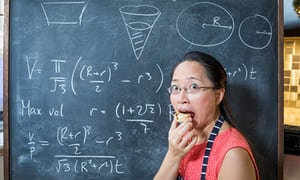
\includegraphics[width=0.35\textwidth]{eugenia-cheng}
\end{wrapfigure}

PS: Falls ihr noch ein Weihnachtsgeschenk für euch selbst sucht, können wir das
Buch \emph{How to Bake Pi: An Edible Exploration of the Mathematics of Mathematics}
von Eugenia Cheng empfehlen. Cheng ist eine der bekanntesten Forscherinnen auf dem
Gebiet der höherdimensionalen Kategorientheorie. In ihrem Buch stellt sie dieses
Gebiet auf verständliche Art und Weise vor.

PPS: Macht ihr beim Matheadventskalender mit?
https:/$\!$/www.mathekalender.de/

\newpage
\fi\ifmore\repeat

\closein\quelle

\end{document}
